\documentclass[12pt,letterpaper,noanswers]{exam}
\usepackage[usenames,dvipsnames,svgnames,table]{xcolor}
\usepackage[margin=0.9in]{geometry}
\renewcommand{\familydefault}{\sfdefault}
\usepackage{multicol}
\usepackage{wrapfig}
\pagestyle{head}
\definecolor{c03}{HTML}{FFDDDD}
\header{AM 22b Class 28}{}{Apr 7: Divergence theorem, p.\thepage}
\runningheadrule
\headrule
\usepackage{graphicx} % more modern
\usepackage{amsmath} 
\usepackage{amssymb} 
\usepackage{hyperref}
\usepackage{tcolorbox}
\usepackage[utf8]{inputenc}
\usepackage{diagbox}
\usepackage{graphicx} 
\usepackage{enumitem}
\usepackage{tikz}
\tikzstyle{startstop} = [rectangle, rounded corners, minimum width=3cm, minimum height=1cm,text centered, draw=black]

\tikzstyle{process} = [rectangle, minimum width=3cm, minimum height=1cm, text centered, draw=black, fill=gray!20]
\tikzstyle{decision} = [ellipse, minimum width=3cm, minimum height=0.5cm, text centered, draw=black, fill=white!30]
\tikzstyle{arrow} = [thick,->,>=stealth]
\usetikzlibrary{shapes.geometric, arrows}
\pagenumbering{arabic}

\usepackage[numbered,autolinebreaks,useliterate]{mcode}

\newcommand{\mb}[1]{\underline{#1}}

\begin{document}
 \pdfpageheight 11in 
  \pdfpagewidth 8.5in




% I need to review the torus trajectories...

\begin{itemize}
% \item There is a pre-class assignment (20 minutes of videos + a few WeBWorK exercises) due at 10am this Monday.  It is available on Canvas.
\itemsep0em
\item There will be a skill check on Monday for C27, 28, 29.
\item Problem set 08 is due on Thursday April 8th at 6pm.
\item There will be a pre-class assignment for Monday.
\end{itemize}

\hrule
\vspace{0.2cm}

% partial derivatives, gradient
% local linearity, differential, directional deriv
% 2nd order partials + equations with partials

\noindent\textbf{Big picture}

For the flux out of a closed surface (or curve) we will have a theorem similar to Green's theorem, where we will integrate the flux density (the divergence) over a region to find the flux out the boundary of the region.  We will work with this divergence theorem today.

\vspace{0.2cm}
\hrule
\vspace{0.2cm}

\noindent\textbf{Skill Check C28 Practice}

 Find the flux of $\underline F = (x+3e^{yz})\mb i + (\ln(x^2z^2+1)+y)\mb j + z\mb k$ out of the closed solid cylindrical region of radius $2$ centered on the $z$-axis, $0\leq r\leq 2$, $3\leq z \leq 7$.

\vspace{0.2cm}
\hrule
\vspace{0.2cm}

\noindent\textbf{Skill Check C28 Practice Solution}

Using the divergence theorem, $\nabla\cdot \underline F = 1 + 1 + 1 = 3$ so the flux is $\int_W 3dV = 3\int_W dV$.  
$3\int_W dV = 3\int_0^{2\pi}\int_0^2\int_3^7 rdzdrd\theta = 12\int_0^{2\pi}\int_0^2 rdr = 24\int_0^{2\pi}d\theta = 48\pi$

\vspace{0.2cm}
\hrule
\vspace{0.2cm}

\noindent\textbf{Teams}
\begin{multicols}{2}

1.  students here
\end{multicols}



\vspace{0.2cm}
\hrule
\vspace{0.2cm}
\noindent\textbf{Flux density (divergence) for 2D vector fields} \S 19.3, \S 18.4
\begin{tcolorbox}
\begin{itemize}
\itemsep0em
    \item The \textbf{divergence} is a measure of the local spread of an infinitesimal region under the action of the vector field.
    \item The \textbf{divergence} of a vector field $\mb F = \langle P,Q,R\rangle$ is given by $\text{div }\mb F = \frac{\partial P}{\partial x}+\frac{\partial Q}{\partial y}+\frac{\partial R}{\partial z}$.  Thinking of the operator $\nabla$ as $\nabla = \langle \frac{\partial }{\partial x},\frac{\partial}{\partial y},\frac{\partial}{\partial z}\rangle$, we can write $\text{div }\mb F = \nabla \cdot \mb F$.
    %\item Let $\displaystyle\mb F = M\mb i + N\mb j$.  $\oint_C \mb F \cdot \mb n ds = \oint_C \mb F \cdot \langle dy, -dx\rangle$.  Rearrange and use Green's theorem to find a flux form of Green's theorem: $\displaystyle\oint_C \mb F \cdot \mb n ds=\oint_C Mdy-Ndx = \oint_C \langle -N, M\rangle \cdot \mb T ds = \int_R (M_x + N_y) dA$.
\end{itemize}
\end{tcolorbox}

\noindent\textbf{Example (vector fields with constant divergence)}

Each of the following four vector fields  has constant divergence everywhere in space.  Identify whether the divergence is positive, negative, or zero.
%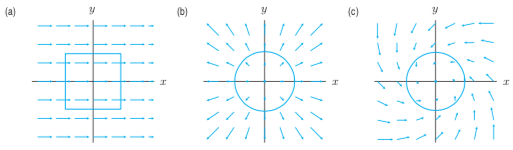
\includegraphics[scale=0.8]{img/C24p1.png}

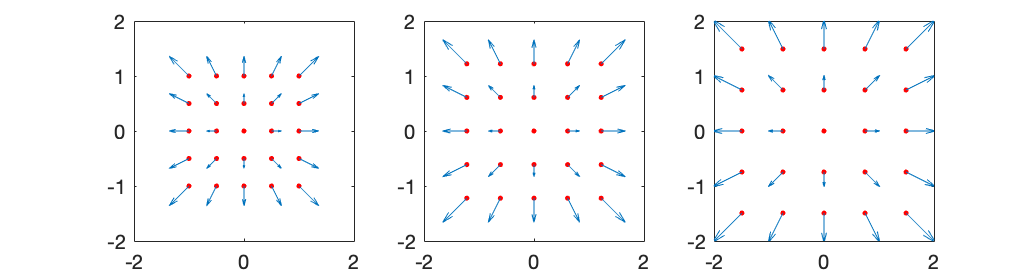
\includegraphics[width=0.9\linewidth]{img/C26p1a.png}

%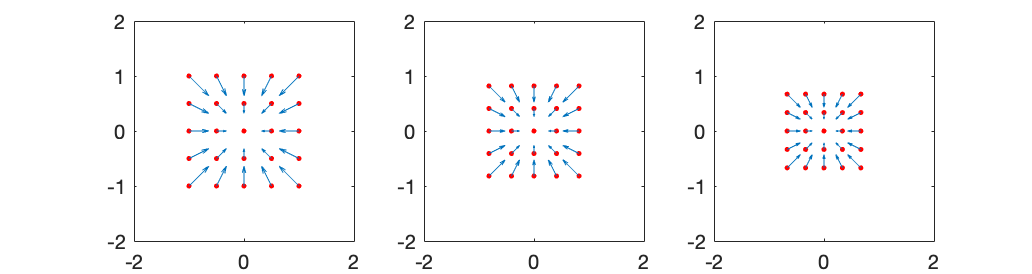
\includegraphics[width=0.9\linewidth]{img/C26p1b.png}

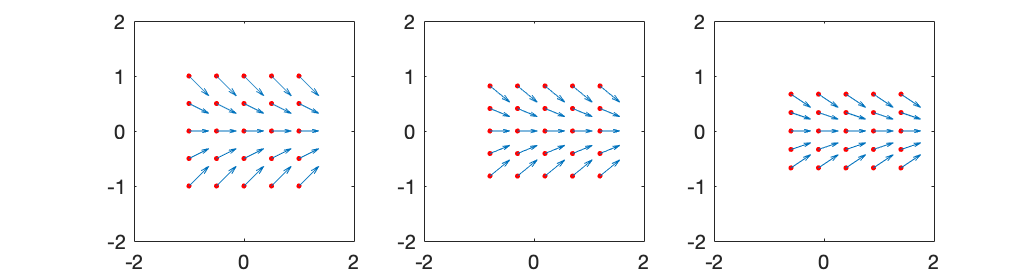
\includegraphics[width=0.9\linewidth]{img/C26p1c.png}

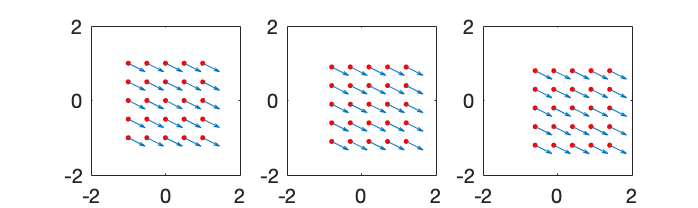
\includegraphics[width=0.9\linewidth]{img/C26p1d.png}

\begin{tcolorbox}
\begin{itemize}
\itemsep0em
    \item \textbf{Divergence free} vector fields are sometimes called \emph{solenoidal}.  (Solenoid is a word associated with a particular kind of electromagnet).  The magnetic field (a vector field from physics) is divergence free.
    \item Divergence free vector fields are sometimes called \textbf{incompressible}.  This term is associated with fluid dynamics and is used for fluids (like water) that are modeled as not stretching or compressing parcels of the fluid while they flow under the action of the vector field.
    \item Divergence is sometimes described as the extent to which a vector field behaves like a \textbf{source} at a given point (positive divergence), or like a \textbf{sink} (negative divergence).
\end{itemize}
\end{tcolorbox}

\noindent\textbf{Example (computing divergence)}
Compute the divergence for the following vector fields.
\begin{enumerate}
\itemsep3em
    \item $-y\mb i + x\mb j$
    \item $3x^2\mb i - \sin(xz)(\mb i + \mb k)$
    \item $\mb r - \mb a$ for $\mb a$ a constant vector field (and $\mb r = \langle x,y,z\rangle$.
    \item $\mb a\times \mb r$ for $\mb a$ a constant vector field
    \vspace{1.3in}
\end{enumerate}





\vspace{0.2cm}
\hrule
\vspace{0.2cm}

\noindent\textbf{Computing flux via the divergence theorem} \S 19.4
\begin{tcolorbox}
\begin{itemize}
\itemsep0em
    \item 3D: The \textbf{divergence theorem}: If $W$ is a solid region whose boundary, $S=\partial W$, is a piecewise smooth surface, and if $\vec F$ is a smooth vector field on an open region containing $W$ and $S$, then $\displaystyle \int_S \vec F\cdot d\vec A = \int_W \text{div }\vec F\ dV$, where $S$ is oriented outward.  
    \item 2D: If $R$ is a region in $2$-space whose boundary, $C = \partial R$ is a piecewise smooth curve, and if $\vec F$ is a smooth vector field on an open region containing $R$ and $C$, then $\displaystyle \int_C \vec F\cdot \underline n\ ds = \int_R \text{div }\vec F\ dA$, where $C$ is oriented outward.
    \item Integrating the divergence over the region $W$ (or $R$) returns the flux out the boundary of the region $\partial W$ (or $\partial R$).  That means the divergence can be interpreted as the flux density: the flux per unit volume (or flux per unit area).
    \item Intuitively, the \textbf{boundary} of a solid region, $\partial W$, is the ``skin'' between the interior of the region and the space surrounding the region.
    \item When a surface is the boundary of a solid region it is called a \emph{closed surface}.  We often use the term `closed' to refer to a set that contains its boundary points.  Instead, here `closed' is being used analogously to `closed curve' (which indicates a curve that makes a full loop).
\end{itemize}


\end{tcolorbox}
\noindent\textbf{Example (traffic on a highway)}.  Consider the traffic on a highway going in a single direction.  At each point on the road, $c(x)\mb i$ cars per hour travel across that point at time zero.  This is a time-dependent vector field (the number of cars per hour traveling across a point changes over time), and we'll consider the vector field at a single instant.  Suppose that at time zero the traffic is steadily slowing down over a five mile length of road (mile $0$ to mile $5$).

%cars move at velocity $M(x)\vec i$ when they reach that point, so the vector field is $\mb v(x) = M(x)\mb i$, defined along the $x$-axis.  If traffic is steadily slowing down as we move in the positive $x$ direction, the cars are cars converging together.

At this instant, $c(0)$ cars per hour enter at mile zero.  $c(5)$ cars per hour exit at mile five.  With traffic slowing down over the length of the road, $c(5)-c(0)$ is negative, with more cars entering the stretch of road than are leaving.  This corresponds to an inward flux of cars of $c(5)-c(0)$ cars per hour entering the region.  \emph{Note that this is unsustainable: on average, all of the cars that enter a stretch of road need to also leave it, so the average flow in at $c(0)$ across all times needs to be balanced by the average flow out at $c(5)$.  However, at the instant the traffic is slowing, more cars enter the stretch of road than leave.}

The divergence theorem says that the divergence of the cars is related to the rate at which cars enter the region.  The divergence is $\frac{dc}{dx}$.  The divergence theorem states that $\displaystyle c(5) - c(0) = \int_0^5 \frac{dc}{dx}dx$.  In this 1D case, this is identical to the fundamental theorem of calculus.

\vspace{0.9in}

\noindent\textbf{Example (going to class)}.  Vector fields can be time dependent.  Think of a vector field describing the flow of students in space.  Just before class starts, students flow into a classroom.  Just after it ends, they flow out.  At $t = 0$, students are flowing into the classroom, so the flux out of the room is negative.  Think of the classroom as a 2D region, with a curve for its boundary.  The divergence theorem tells us that the integral of the divergence within the classroom, $\int_{\text{classroom}} \nabla \cdot \underline v\ dA$, is exactly equal to the flux out the boundary of the classroom, $\int_{\partial \text{classroom}} \underline v \cdot \underline n\ ds$.  

\vspace{1in}

\noindent\textbf{Question (divergence free vector fields)}.  Let $\vec F$ be a smooth vector field defined everywhere in $3$-space.  Let $\vec F$ be divergence free.  Let $W$ be a solid region.  What is the flux through the boundary of $W$, $\partial W$?

\vspace{1.5in}

\noindent\textbf{Question (zero flux)}.  Let $W$ be a solid region.  Let $\underline F$ be a smooth vector field defined everywhere in $3$-space.  Assume $\underline F$ has zero flux through the boundary of $W$, $\partial W$.

Mark the following statement as true or false: $\nabla \cdot \underline F = 0$ everywhere in $W$.
\vspace{1in}

\noindent\textbf{Example (sphere)}.  In a previous class, we set up a flux integral to find the flux of $\vec F = \vec r$ outward through $S$ where $S$ was the sphere of radius $a$, centered at the origin and oriented outward.  We had $\displaystyle \int_S \vec F\cdot d\vec A = \int_0^{2\pi}\int_0^{\pi} \vec r\cdot \frac{\vec r}{a} \ a^2\sin\phi\  d\phi\ d\theta = \int_0^{2\pi}\int_0^{\pi} a \ a^2\sin\phi\  d\phi\ d\theta = a\text{ Area}(S)$.
Use the divergence theorem to calculate this flux.
\begin{enumerate}
\itemsep3em
    \item Find $\vec\nabla \cdot \vec F$.
    \item Set up the integral $\int_W \vec\nabla \cdot \vec F\ dV$.
    \item Integrate.
    \vspace{1in}
\end{enumerate}


\noindent\textbf{Question (cylinder)}.  Let $S_1$ be the cylindrical surface given by $r = 2, 0\leq \theta\leq 2\pi, 0\leq z\leq 3$.  Let $D_1$ be the disk of radius $2$ in the $xy$-plane, centered at the origin and oriented downward.  Let $D_2$ be the disk of radius $2$ in the plane $z=3$, centered at the origin and oriented upward.  

Use the divergence theorem to compute the flux of $\vec F = xz\vec i + yz\vec j + z^3\vec k$ through $D_1+D_2+S_1$.

\vspace{3in}


\noindent\textbf{Example (flux through disk)}.  Let $D_1$ ($z=0$) and $D_2$ ($z=2$) be disks defined as above.  Compute the flux of $\vec F = xz\vec i + yz\vec j + z^3\vec k$ down through $D_1$, and the flux up through $D_2$.  

\vspace{2in}


\noindent\textbf{Example (flux through the cylindrical surface)}.  For the surfaces defined above, find the flux outward through the cylindrical surface $S_1$.
\vspace{1.5in}



\noindent\textbf{Summary (cylindrical can)}.  Let $W$ be the solid cylindrical region given by $r\leq 2, 0\leq z\leq 3, 0\leq \theta\leq 2\pi$.  $\partial W = S_1+D_1+D_2$ (so long as everything is oriented carefully to match the outward direction for $\partial W$).

\[\displaystyle \int_W \vec\nabla\cdot\vec F\ dV = \int_{S_1}\vec F\cdot d\vec A + \int_{D_1}\vec F\cdot d\vec A + \int_{D_2}\vec F\cdot d\vec A.\]

\[\displaystyle  \int_{S_1}\vec F\cdot d\vec A = \int_W \vec\nabla\cdot\vec F\ dV - \int_{D_1}\vec F\cdot d\vec A - \int_{D_2}\vec F\cdot d\vec A.\]


\vspace{0.5cm}


\vspace{0.2cm}
\hrule
\vspace{0.2cm}

% \noindent\textbf{Regions with a hole in them} \S 19.4, \S 18.4
% \begin{tcolorbox}
% \begin{itemize}
% \itemsep0em
%     \item Consider a vector field $\underline F$ that is defined and smooth everywhere on $S = \partial W$ but that is not defined at some point within $W$.  We cannot use the divergence theorem.  Something very similar happened the Green's theorem.
%     \item When there is a hole in $R$ (with $C = \partial R$) or in $W$ (with $S = \partial W$), enclose the hole with a circle/square or sphere/cube (depending on the dimension).  Make the curve/surface you choose small enough that it is completely contained within $R$ or $W$.  
%     \item Choose whatever curve/surface is easiest to compute your integral.  Directly compute the circulation on that curve or flux out that curve/surface.
%     \item Use the Divergence theorem or Green's theorem on the region in between your curve/surface and $C$ or $S$.  This will be a region with an ``inner boundary'' and an ``outer boundary''.  
%     \item In the special case when the vector field is curl-free or divergence-free away from the hole, the circulation on $C$ or the flux out $C$ or $S$ will exactly match the value on the surface you've made up.
% \end{itemize}

% \end{tcolorbox}

% \noindent\textbf{Hole at the origin.} According to Coulomb's Law, the electric field produced by a point charge $q$ placed at the origin is $\displaystyle \vec F = \frac{q}{\Vert \vec r\Vert^2}\frac{\vec r}{\Vert \vec r\Vert}$.  This vector field is undefined at the origin.  Away from the origin, it is divergence free.


% Calculate $\int_S \vec F\cdot d\vec A$ for the following surfaces:
% \begin{itemize}
%     \item $S_1$ is the sphere of radius $a$ centered at the origin, oriented outward.  \emph{The divergence theorem does not apply on the $W$ where $\partial W = S_1$ because $\vec F$ and $\vec\nabla \cdot \vec F$ are undefined at the origin, so a flux integral is required.}
%     \item $S_2$ is the ellipsoid $x^2+y^2+4z^2 = 16$, oriented outward.  \emph{Consider the surface $S_2 - S_1$ (for $a = 1$.)  A cut-away view of $S_2 - S_1$ is shown below.  Let $W$ be the region in between, with $\partial W = S_2 - S_1$.}
% \end{itemize}

% 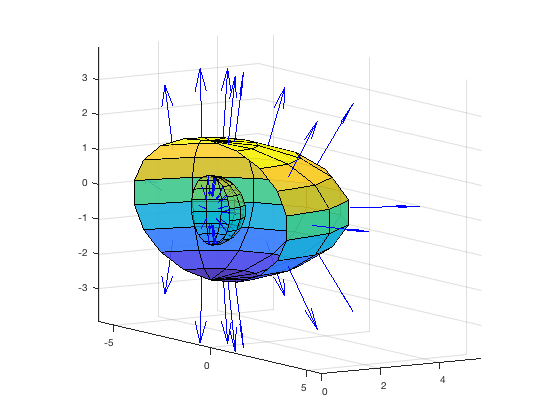
\includegraphics[width=3in]{img/C32p4-18.png}





\end{document}